% CVPR 2022 Paper Template
% !TEX root = PaperForReview.tex
\documentclass[12pt,letterpaper]{article}

\usepackage{cvpr}
\usepackage{titling}
\usepackage{enumitem}
\usepackage{graphicx}
\usepackage{amsmath}
\usepackage{amssymb}
\usepackage{booktabs}
\usepackage{CJKutf8}
\usepackage{geometry}
\usepackage{float}
 \geometry{
 a4paper,
 total={170mm,257mm},
 left=20mm,
 top=20mm,
 }
%  \setlength{\headheight}{15.0pt}
\addtolength{\topmargin}{-3.0pt}

\usepackage[pagebackref,breaklinks,colorlinks]{hyperref}
% \usepackage{fancyhdr}
% \fancypagestyle{plain}{%  the preset of fancyhdr 
%     \fancyhf{} % clear all header and footer fields
%     \fancyhead[L]{Computer Vision Homework 1 Report}
%     \fancyhead[R]{\today}
% }
\makeatletter
% Support for easy cross-referencing
\usepackage[capitalize]{cleveref}
\crefname{section}{Sec.}{Secs.}
\Crefname{section}{Section}{Sections}
\Crefname{table}{Table}{Tables}
\crefname{table}{Tab.}{Tabs.}
\newcommand{\xeq}[1]{Eq.~(\ref{#1})}
\newcommand{\xeqs}[2]{Eqs.~(\ref{#1}) and~(\ref{#2})}
\newcommand{\xkw}[1]{\textcolor{blue}{\textbf{#1}}}
\newcommand{\xfig}[1]{Figure~\ref{#1}}
\newcommand{\xfigx}[2]{Figures~\ref{#1}--\ref{#2}}
\newcommand{\xfigs}[2]{Figures~\ref{#1} and~\ref{#2}}
\newcommand{\xfigss}[3]{Figures~\ref{#1}, \ref{#2}, and~\ref{#3}}
\newcommand{\xfigsss}[4]{Figures~\ref{#1}, \ref{#2}, \ref{#3}, and~\ref{#4}}
\newcommand{\xsubfig}[1]{Figure~\ref{#1}}
\newcommand{\xsubfigs}[1]{Figures~\ref{#1}}
\newcommand{\xtab}[1]{Table~\ref{#1}}
\newcommand{\xtabs}[2]{Tables~\ref{#1} and~\ref{#2}}
\newcommand{\xtabss}[3]{Tables~\ref{#1}, ~\ref{#2}, and~\ref{#3}}
\newcommand{\xtabt}[2]{Tables~\ref{#1} through~\ref{#2}}
\newcommand{\xsec}[1]{Section~\ref{#1}}
\newcommand{\xalg}[1]{Algorithm~\ref{#1}}
\newcommand{\xalgs}[2]{Algorithms~\ref{#1} and~\ref{#2}}
\newtheorem{dpd}{Definition}
\newtheorem{xdefinition}{Definition}
\newcommand{\opt}{\mathop{\rm optimize}}
\newcommand{\subject}{\mathop{\rm subject~to}}
\newcommand{\xdf}[1]{Definition~\ref{#1}}

\newcommand{\xmetah}{metaheuristic}
\newcommand{\xmetahs}{metaheuristics}
\newcommand{\xmetaha}{metaheuristic algorithm}

\newcommand{\xPropose}{AdaMMP}
\newcommand{\xProposeFull}{Adaptive Multi-Metric Predictor}
\newcommand{\xProposeP}{\xPropose~proxy}
\newcommand{\xNAS}{neural architecture search}
\newcommand{\xnasblol}{NAS-bench-101}
\newcommand{\xnasbtss}{NAS-bench-201}
\newcommand{\xnasbsss}{NATS-bench-SSS}

\newcommand{\xq}[1]{\textcolor{red}{#1}}
\newcommand{\xqq}[1]{\textcolor{red}{\sout{#1}}}
% \newcommand{\xr}[1]{\label{#1}\textcolor{red}{(#1)}}
\newcommand{\xr}[1]{\label{#1}}
% \newcommand{\xs}[1]{\textcolor{magenta}{#1}}
\newcommand{\xs}[1]{#1}
\newcommand{\xt}[1]{\textcolor{black}{#1}}
\newcommand{\xx}[2]{{#2}}

\usepackage[normalem]{ulem}
\newcommand{\xold}[1]{\textcolor{red}{#1}} % original text
\newcommand{\xnew}[1]{\textcolor{blue}{#1}} % replacement text
\newcommand{\xch}[2]{\xqq{#1} \xnew{#2}}

% \newcommand{\xfig}[1]{圖~\ref{#1}}
% \newcommand{\xfigs}[2]{圖~\ref{#1} and~\ref{#2}}
% \newcommand{\xq}[1]{\textcolor{red}{#1}}

% \newcommand{\xmold}[1]{\textcolor{red}{#1}} % original text
% \newcommand{\xmnew}[1]{\textcolor{blue}{#1}} % replacement text
% \newcommand{\xch}[2]{\xmold{\sout{#1}}\xmnew{#2}}

\newcommand{\xAns}{\vskip 2mm\textbf{Answer:} }
\begin{document}
\begin{CJK}{UTF8}{bkai}
    %%%%%%%%% TITLE
    \title{Evolutionary Computation - Homework 1}

    \author{
        高聖傑\\
        313552011\\
    }

    \maketitle
\end{CJK}

\section*{Question 1}
The eight queens problem.
\begin{enumerate}[label=(\alph*)]
    \item How big is the phenotype space for the eight queens problem? \xAns A valid solution for the problem can be considered as a phenotype. There are no known formulas to calculate the exact number of valid solutions for the eight queens problem, so the size of the phenotype space is figured out by counting the number of valid solutions via brute force, DFS, or other methods, which is $92$.
    \item Give a genotype to encode the 8x8 chessboard configuration. \xAns A genotype can be represented by an array of 8 integers, where each integer represents the row index of the queen in the corresponding column.
    \item How big is the genotype space you give in (b)? \xAns Genotype space is the permutation of the integers from 1 to 8, which is $8! = 40320$.
    \item Briefly describe why the proposed genotype is able to cover the phenotype space. \xAns Since the genotype covered all permutations of the integers from 1 to 8, the proposed genotype is able to cover the phenotype space, which is subset of the genotype space.
\end{enumerate}
% \subsection{}
\section*{Question 2}
Given a function $f(x) : [0,1] \rightarrow \mathbb{R}$. We want to find an optimal $x$
value with a required precision of 0.001 of the solution. That is, we
want to be sure that the distance between the found optimum and the
real optimum is at most 0.001. How many bits are needed at least to
achieve this precision for a bit-string genetic algorithm?
\xAns The required precision means that the distance between the found optimum and the real optimum is at most 0.001. The number of bits needed to achieve this precision can be calculated as follows:
\begin{equation}
    2^{-n} \leq 0.001
\end{equation}
where $n$ is the number of bits. Solving for $n$ gives:
\begin{equation}
    n \geq = \log_2(1000) \approx 9.966
\end{equation}
Therefore, at least 10 bits are needed to achieve a precision of 0.001 for a bit-string genetic algorithm.
\section*{Question 3 \& 4}
OneMax problem with genetic algorithm, using roulette wheel selection.
\begin{figure}[H]
    \centering
    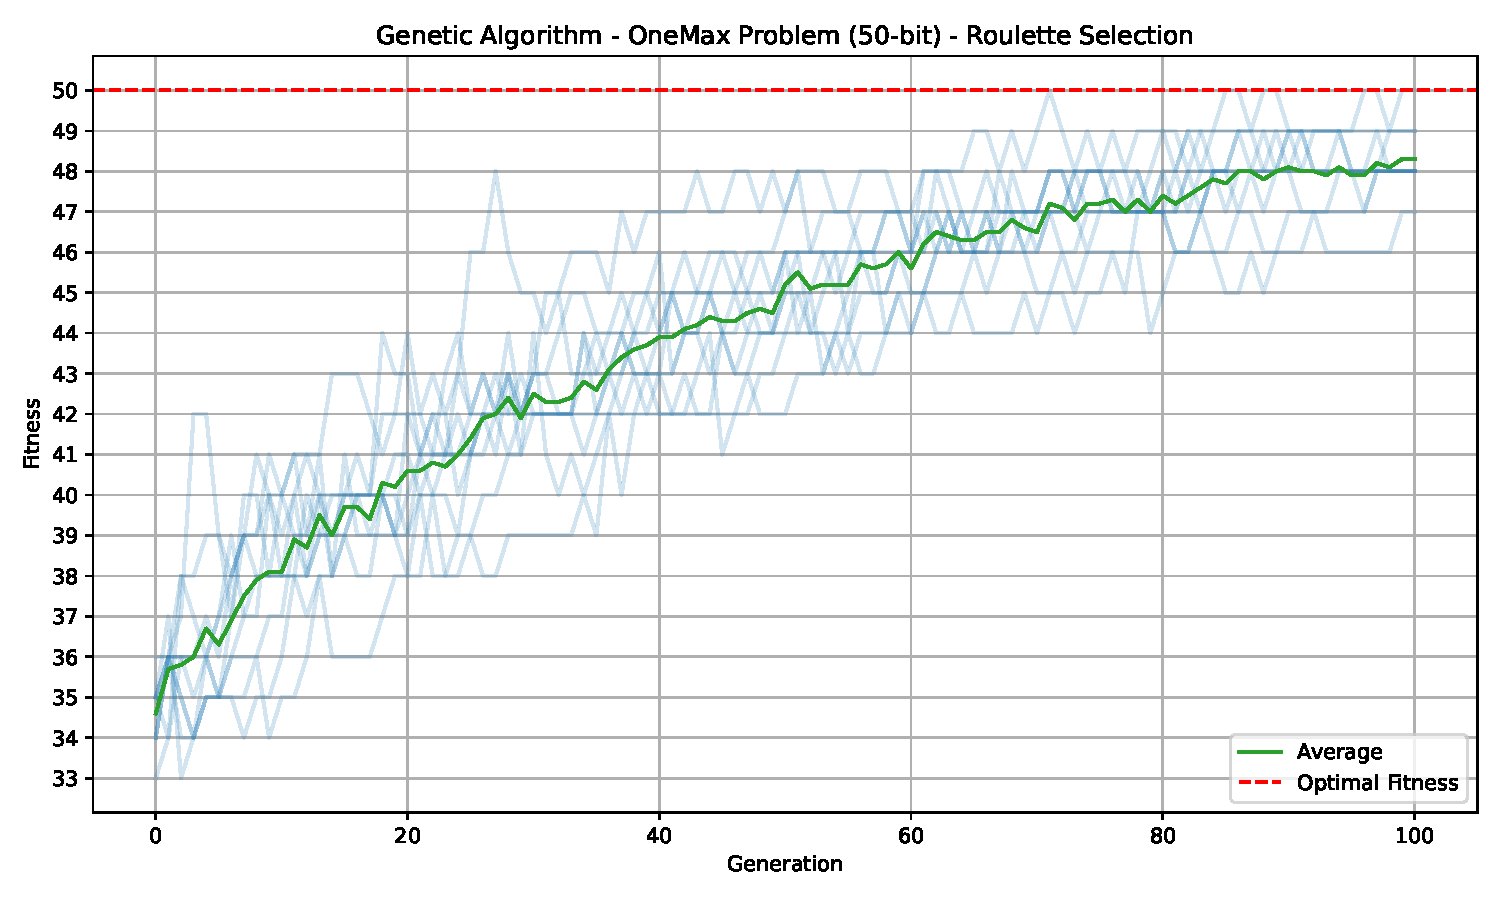
\includegraphics[width=0.8\textwidth]{images/oneMax_GA_roulette.pdf}
    \caption{Best and average of best fitness over generations, using roulette wheel selection.}
    \label{fig:3a}
\end{figure}
Modified fitness function.
\begin{figure}[H]
    \centering
    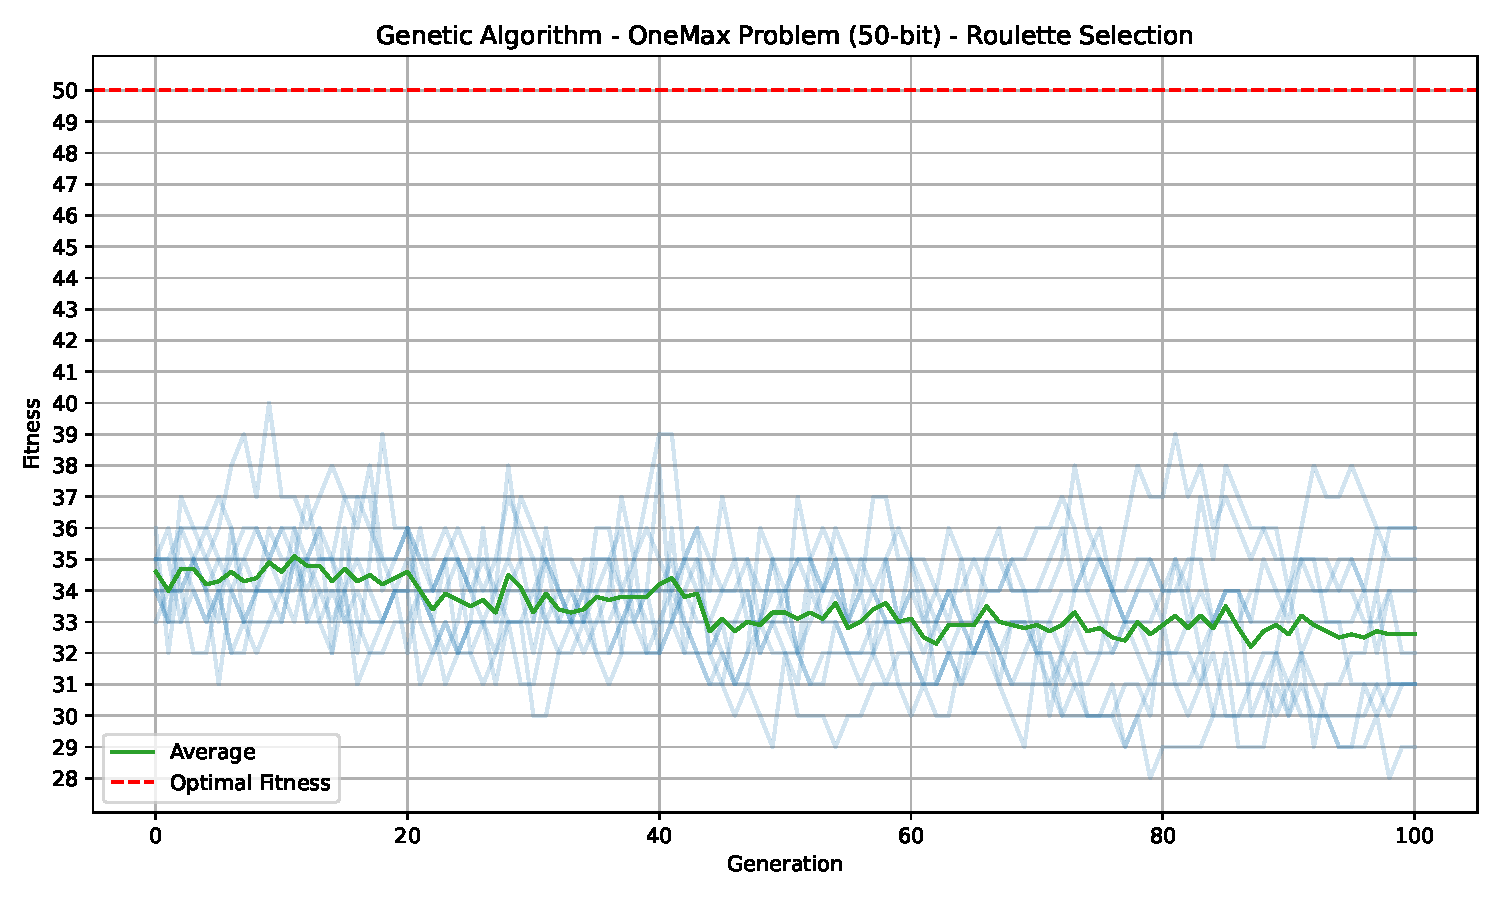
\includegraphics[width=0.8\textwidth]{images/oneMax_GA_roulette_mod.pdf}
    \caption{Best and average of best fitness over generations, using roulette wheel selection with the modified fitness function.}
    \label{fig:4a}
\end{figure}

\section*{Question 5}
Compare Question 3 and 4. \xAns In \xfigs{fig:3a}{fig:4a}, we can observe that adding 1000 to fitness values when selecting parents made devastating impact on the performance of the genetic algorithm. The reason is that the chances of selecting an individual in the roulette method are proportional to the ratio of each individual's fitness to the sum of fitness. When you add a constant to each individual's fitness, which make the relative fitness difference between the individuals becomes relatively small, it becomes even more difficult to tell good individuals from bad ones. As a result, the selection process now has lower selection pressure, relies more on randomness, and the superior individuals do not get enough advantage, which in turn reduces the quality of the solution.

\section*{Question 6 \& 7}
OneMax problem with genetic algorithm, using tournament selection.
\begin{figure}[H]
    \centering
    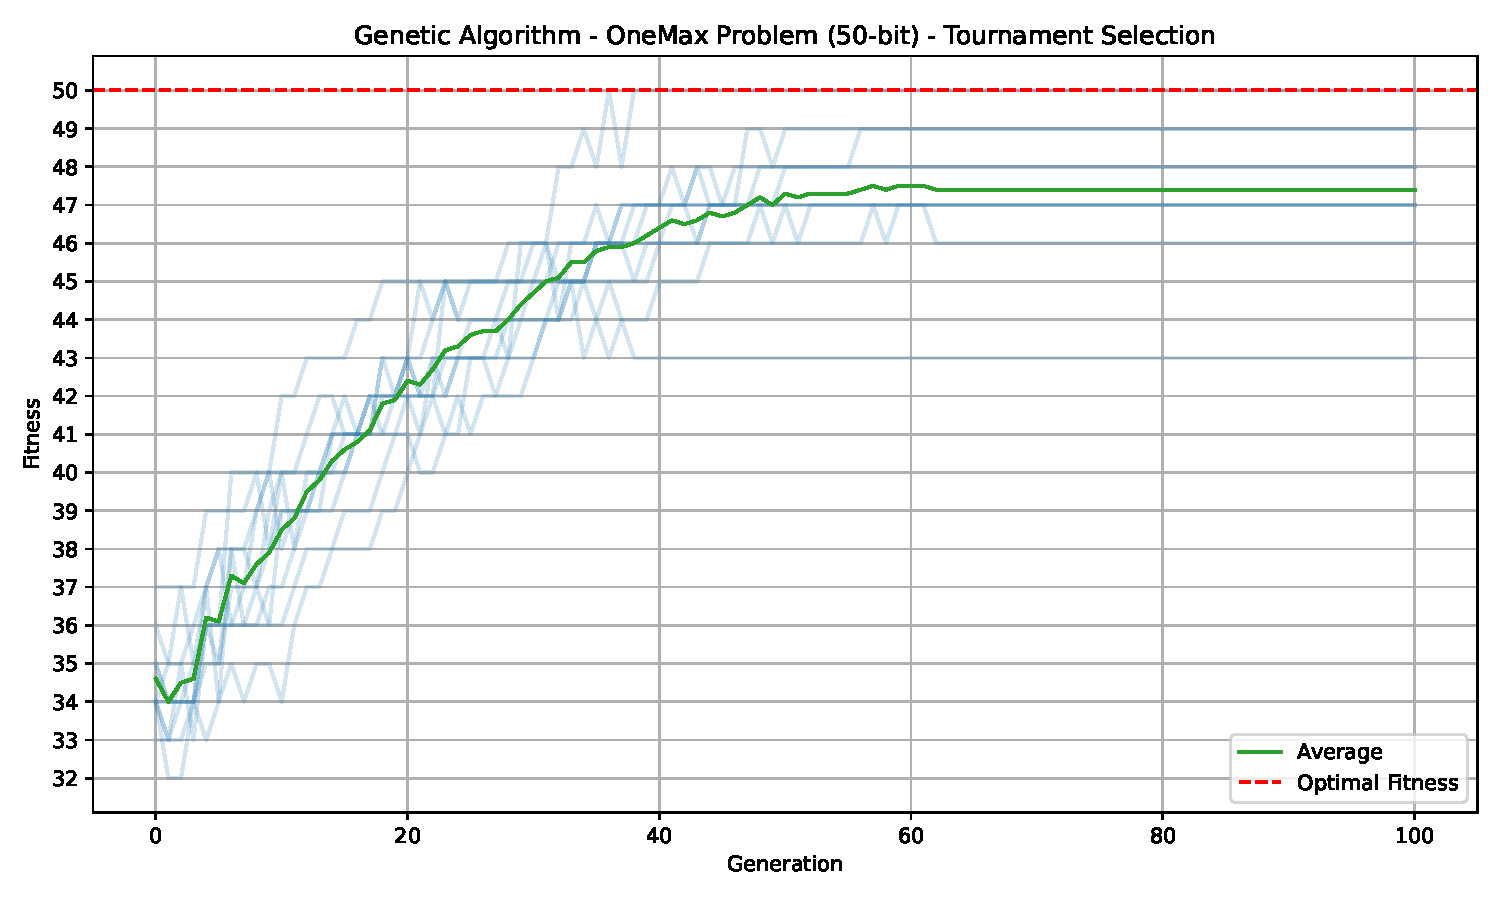
\includegraphics[width=0.8\textwidth]{images/oneMax_GA_tournament.pdf}
    \caption{Fitness of each run and the average fitness of the population over generations, using tournament selection.}
    \label{fig:6a}
\end{figure}
Modified fitness function.
\begin{figure}[H]
    \centering
    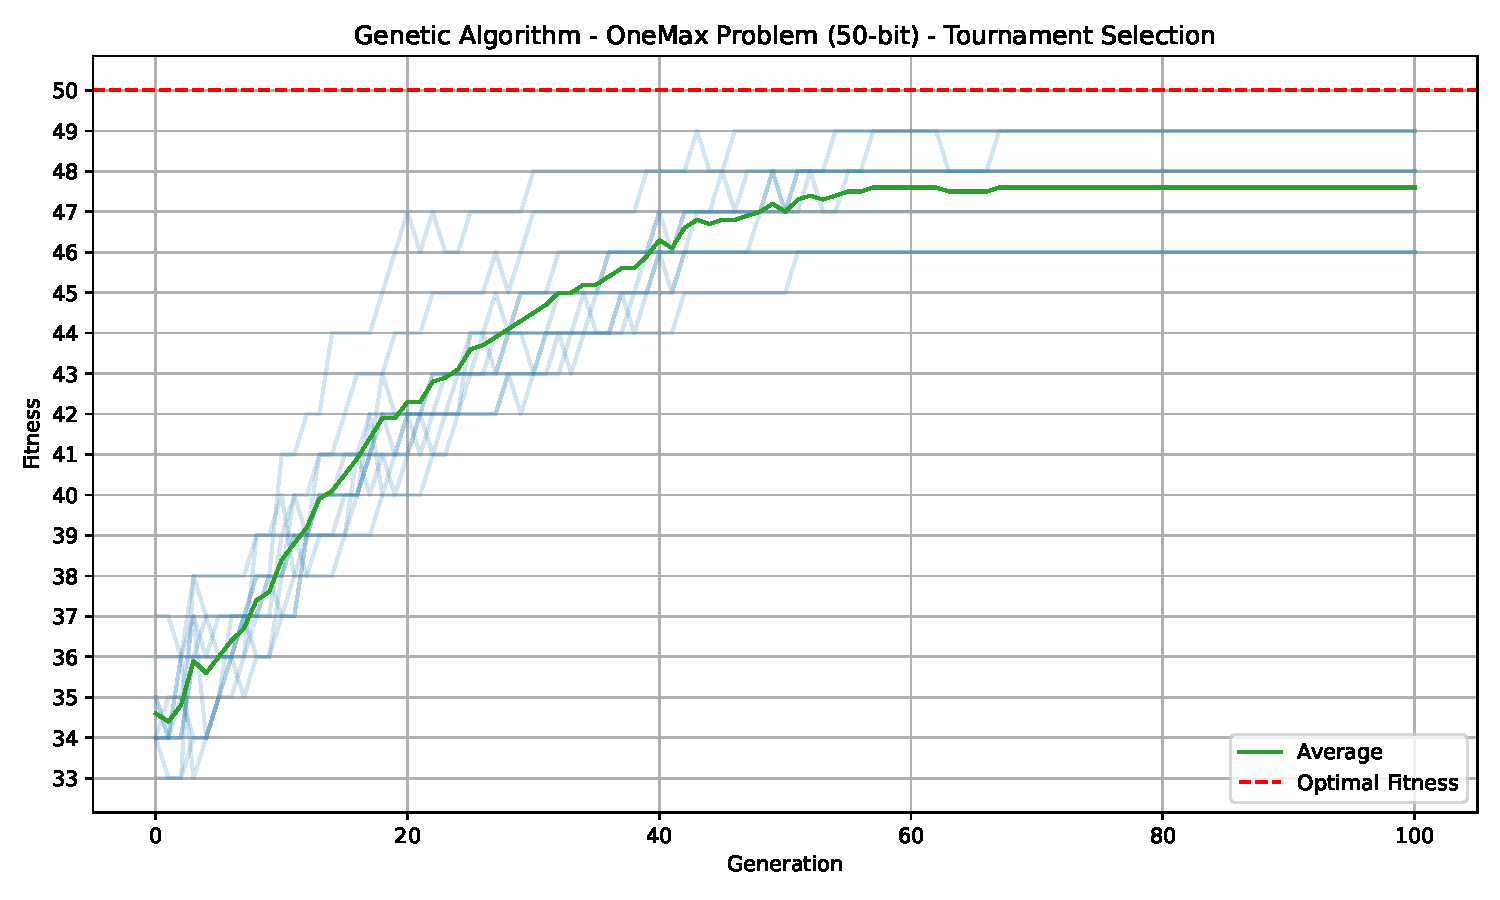
\includegraphics[width=0.8\textwidth]{images/oneMax_GA_tournament_mod.pdf}
    \caption{Fitness of each run and the average fitness of the population over generations, using tournament selection with the modified fitness function.}
    \label{fig:7a}
\end{figure}
\section*{Question 8}
Compare Question 6 and 7. \xAns In \xfigs{fig:6a}{fig:7a}, we can observe that adding 1000 to fitness values does not make much difference in the performance when using tournament selection. The reason is that the tournament selection method is less sensitive to the absolute fitness values of the individuals, as adding a constant to the fitness values does not change the ranking of the individuals.

\section*{Question 9}
Compare Question 3, 4, 6, and 7. \xAns Comparing \xfigs{fig:3a}{fig:6a}, with the original fitness function, we can observe that the tournament selection converges faster and has less deviation than the roulette wheel selection, which aligns with the greedy selection property of the tournament selection. On the other hand, the roulette wheel selection relies more on relative fitness differences, making it difficult to distinguish between individuals at the point of where all individuals are close to the optimum. 
\begin{figure}[H]
    \centering
    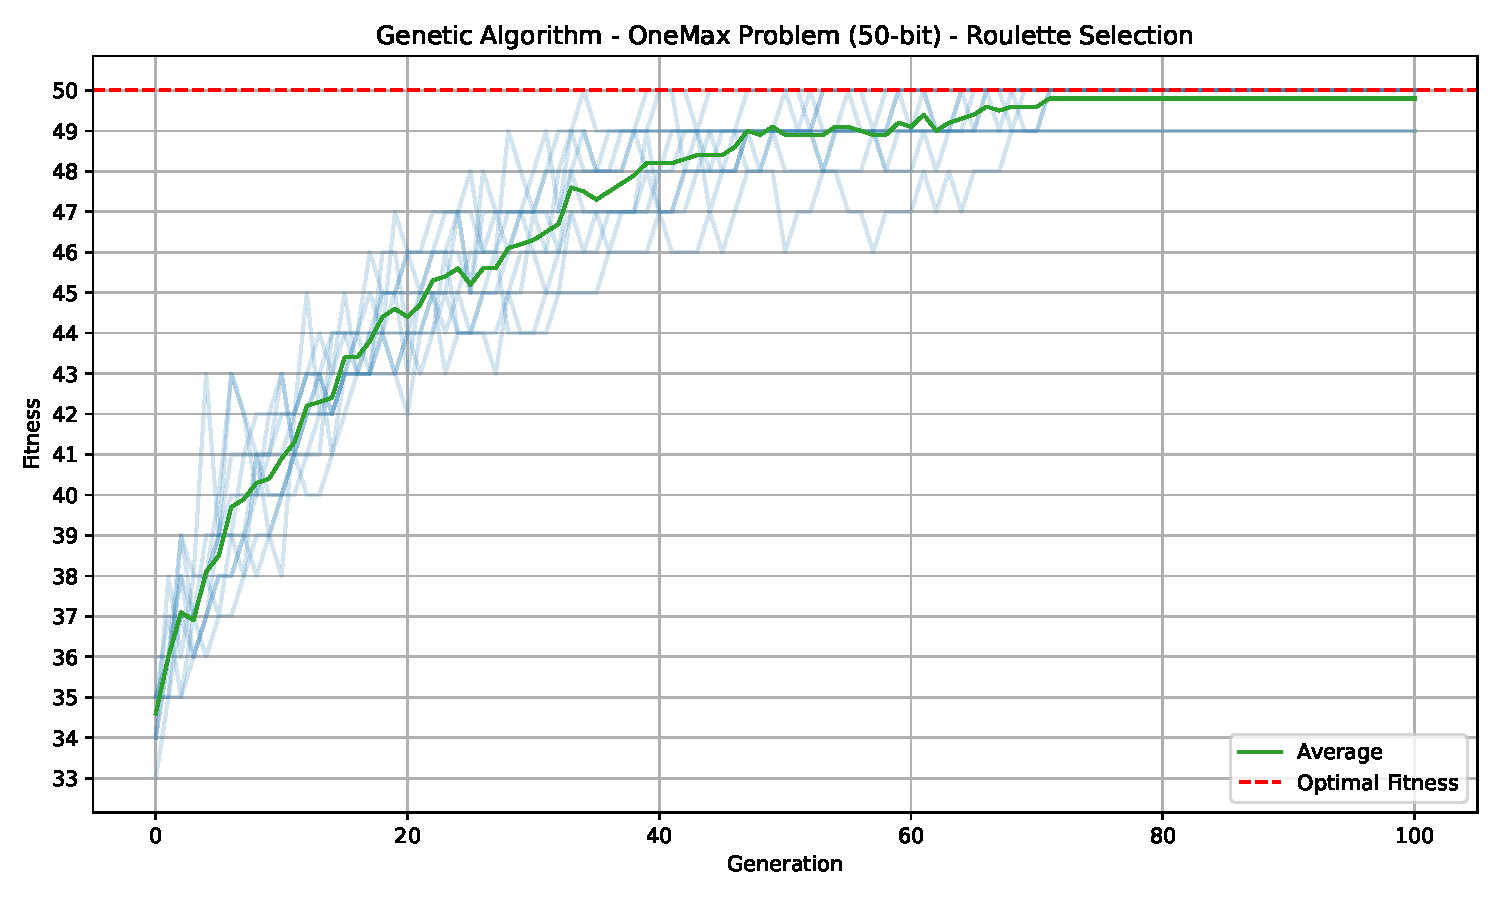
\includegraphics[width=0.8\textwidth]{images/oneMax_GA_roulette_fs.pdf}
    \caption{Best and average of best fitness over generations, using roulette wheel selection with fitness scaling.}
    \label{fig:9a}
\end{figure}
As shown in \xfig{fig:9a}, fitness scaling can be introduced to the roulette wheel selection to improve its performance, by using a nonlinear conversion, which is simply squaring the fitness values in this case, a better performance can be achieved.

In \xfigs{fig:4a}{fig:7a}, with the modified fitness function, we can observe that the tournament selection is unaffected by the modification, while the roulette wheel selection is severely impacted, this implies that the roulette wheel selection need to be carefully designed to handle the fitness scaling issue.
\end{document}